% !TEX root = ./main.tex
\documentclass[bigger,notes]{beamer}
\usetheme{metropolis}
\title{Bridging the gap between Typestates and Rust in production code}
\author{\textbf{José Duarte}\texorpdfstring{\\ António Ravara (Advisor)}{}}
\date{March 2021}
\institute{NOVA School of Science and Technology}

\usepackage{tikz}
\usetikzlibrary{shapes,backgrounds,positioning}
\usepackage{xcolor}

\usepackage{pgfpages}
\usepackage{hyperref}
% \usepackage{listings}
% \lstset{
%     basicstyle=\small\ttfamily,
%     frame=single,
%     % numberstyle=\tiny,
%     % numbers=left
% }

\usepackage{amssymb}


\usepackage[newfloat]{minted}
\setminted{
    linenos,
    frame=single,
    style=lovelace,
    fontsize=\small,
}

\usepackage[main=american,portuguese]{babel}
\babeltags{pt=portuguese, enUS=american}

\setbeameroption{show notes on second screen}

\begin{document}

\begin{frame}[plain]
    \titlepage

    \note{
        \begin{pt}
            Bom dia Professor(es), sou o José Duarte, e o meu tema de tese é "Bridging the gap between typestates and Rust in production code".

            O tema é orientado pelo Professor António Ravara.
        \end{pt}
    }
\end{frame}

\AtBeginSection[]
{
    \begin{frame}
        \frametitle{Outline}
        \tableofcontents[currentsection, hideothersubsections]
    \end{frame}
}

\begin{frame}
    \frametitle{Outline}
    \tableofcontents[hideallsubsections]

    \note{
        \begin{pt}
            Durante a apresentação irei:
            \begin{itemize}
                \item Introduzir o tema.
                \item Rever sumariamente o estado da arte.
                \item Rever um caso de estudo simples, apresentando assim o projeto.
                \item Por fim, falar do plano de trabalho para o semestre.
            \end{itemize}
        \end{pt}
    }
\end{frame}

\section{Introduction}

\note{
    \begin{pt}
        Relativamente à introdução irei:
        \begin{itemize}
            \item Contextualizar o tema da tese.
            \item Apresentar o problema que a mesma visa endereçar.
            \item Os objetivos da tese.
            \item Finalmente, o que são typestates, antes de aprofundar nas secções seguintes.
        \end{itemize}
    \end{pt}
}

\subsection{Context}
\begin{frame}
    \frametitle{Context}
    Software plays a crucial role in our lives.
    \begin{itemize}
        \item From web browsers, to word processors and more!
    \end{itemize}

    As software becomes more important, bugs become more expensive.
    \begin{itemize}
        \item Losing work due to a bug in the save procedure is not nice.
        \item A bug in the firmware for a pacemaker may cost a life.
    \end{itemize}

    \note{
        \begin{pt}
            Dado o papel crescente do software nas nossas vidas,
            os bugs saem cada vez mais caro, tanto às empresas como aos utilizadores.

            Perder uma mensagem no Facebook não é grave, mas um dia de trabalho é pior.
            Imagine-se então um bug num pacemaker, pode causar a morte do utilizador!
        \end{pt}
    }
\end{frame}

\subsection{Problem}
\begin{frame}
    \frametitle{Problem}
    \begin{figure}
        \centering
        \begin{tikzpicture}
            \def\Y{3}
            \def\fstcircle{(0, 0) circle (2.5)}
            \def\sndcircle{(0,-1.25) circle (1)}

            \fill[fill opacity=0.25, blue] \fstcircle;
            \fill[fill opacity=0.35, red] \sndcircle;

            \draw \fstcircle;
            \draw \sndcircle;

            \node at (0, \Y) {Preventable};
            \node at (0, 0.25) {Prevented};
        \end{tikzpicture}
        \caption{Diagram of preventable bugs and prevented bugs.}
    \end{figure}

    \note{
        \begin{pt}
            Podemos imaginar todos os tipos de bugs como um conjunto (não mostrado),
            onde se inserem dois subconjuntos.
            Os bugs que podemos prevenir e os que, de facto, conseguimos prevenir.

            Por exemplo, erros de gestão de memória e mau uso de APIs.
        \end{pt}
    }
\end{frame}

\begin{frame}
    \frametitle{Problem --- with Rust}
    \begin{figure}
        \centering
        \begin{tikzpicture}
            \def\Y{3}
            \def\fstcircle{(0,0) circle (2.5)}
            \def\sndcircle{(0,-.75) circle (1.5)}

            \fill[fill opacity=0.25, blue] \fstcircle;
            \fill[fill opacity=0.35, red] \sndcircle;

            \draw \fstcircle;
            \draw \sndcircle;

            \node at (0, \Y) {Preventable};
            \node at (0, -.75) {Prevented};
        \end{tikzpicture}
        \caption{Diagram of preventable bugs and prevented bugs when considering Rust's borrow checker.}
    \end{figure}

    \note{
        \begin{pt}
            Rust permite-nos alargar o conjunto de bugs que conseguimos prevenir,
            incluindo assim os bugs de memória e de concurrência.

            No entanto, continua a não conseguir cobrir todos os bugs.
        \end{pt}
    }
\end{frame}

\begin{frame}
    \frametitle{Problem --- Ideal}
    \begin{figure}
        \centering
        \begin{tikzpicture}
            \def\X{0}
            \def\fstX{-\X}
            \def\sndX{\X}
            \def\Y{0}
            \def\fstcircle{(\fstX,0) circle (2.5)}
            \def\sndcircle{(\sndX,0) circle (2.5)}

            \fill[fill opacity=0.25, blue] \fstcircle;
            \fill[fill opacity=0.35, red] \sndcircle;

            \draw \fstcircle;
            \draw \sndcircle;

            \node at (\fstX-4, \Y) {Preventable};
            \node at (\sndX+4, \Y) {Prevented};
        \end{tikzpicture}
        \caption{The ideal diagram of preventable bugs and prevented bugs, where all bugs are prevented.}
    \end{figure}
    \note{
        \begin{pt}
            O ideal seria uma sobreposição total, como na figura.
            Os typestates ajudam-nos a dar um passo nesta direção.
        \end{pt}
    }
\end{frame}

\subsection{Objectives}
\begin{frame}
    \frametitle{Objectives}
    A library which brings \emph{practical} typestates to Rust.
    \begin{itemize}
        \item Minimal learning overhead.
        \item Zero-cost abstraction.
        \item Scalable to large projects.
    \end{itemize}

    \note{
        \begin{pt}
            Esta tese visa então providenciar typestates práticos na linguagem Rust.

            Os mesmos:
            \begin{itemize}
                \item Devem ser fáceis de aprender e usar.
                \item Não devem impactar a performance durante o runtime.
                \item Devem escalar a projetos grandes.
            \end{itemize}
        \end{pt}
    }
\end{frame}

\subsection{What are typestates?}
\begin{frame}
    \frametitle{What are typestates?}
    Typestates are an approach to behavioral types.

    They can be modelled as state-machines and allow the developer to cleanly and concisely express API constraints.

    E.g. Java's \texttt{Scanner} cannot be used after being closed.

    Typestates enforce this at compile-time, rather than at runtime.

    \note{
        \begin{pt}
            \footnotesize
            Após esta apresentação de alto nível de typestates, o que afinal são typestates?

            Typestates são uma abordagem a tipos comportamentais.
            Estes visam descrever o estado em runtime do programa através do sistema de tipos.

            Podem ser modelados como máquinas de estados e permitem ao programador expressar de forma clara e consisa restrições de uso de uma API.

            Por exemplo: o famoso \texttt{Scanner} de Java, não pode ser usado depois de ser fechado, no entanto, o compilador não avisa se tal acontecer.
            Só durante o runtime é que uma excepção será lançada.

            Os typestates permitem que o compilador valide este tipo de restrições.
        \end{pt}
    }
\end{frame}

\section{State of the Art}
\note{
    \begin{pt}
        Irei agora efectuar uma breve revisão do estado da arte e de outros projetos existentes.
        Começando por session types e seguindo para typestates.
    \end{pt}
}
\subsection{Session Types}
\begin{frame}
    \frametitle{Session Types --- StMungo}
    StMungo is a tool that converts Scribble local protocols into a Mungo typestate specification and Java skeleton.
    \begin{figure}
        \centering
        \begin{tikzpicture}
            \node (scribble) at (0,  0) {Scribble};
            \node (java)     at (4,  1.25) {Java};
            \node (mungo)    at (4, -1.25) {Mungo};

            \draw[->, thick] (scribble) edge[out=0, in=180] (java);
            \draw[->, thick] (scribble) edge[out=0, in=180] (mungo);
            \draw[->, thick, dashed] (mungo) -- node[right, font=\scriptsize\itshape] {Checks} (java);
        \end{tikzpicture}
    \end{figure}
    Scribble further enables the conversion of multiparty session types into binary session types.
    \note{
        \begin{pt}
            O StMungo (ou Scribble to Mungo) é uma ferramenta que converte protocolos de Scribble para especificações de typestates em Mungo e esqueletos de API em Java.
            A implementação Java é depois verificada pelo Mungo.

            O Scribble permite ainda a conversão de multiparty session types para binary session types.
        \end{pt}
    }
\end{frame}

\begin{frame}
    \frametitle{Session Types --- Session Types for Rust}
    The first work with session types and Rust.

    Exploits the type system to provide binary session types checked at compile-time.

    The library makes use of \texttt{unsafe} features.

    \note{
        \begin{pt}
            (Tanto quanto sei) Esta biblioteca foi a primeira a trazer session types para Rust.

            Tira partido do sistema de tipos para validar as especificações de session types.

            Dado que usa \texttt{unsafe} pode não ser adequada para todos os casos de usos.
        \end{pt}
    }
\end{frame}

\begin{frame}
    \frametitle{Session Types --- Multiparty Session Types for Rust}
    This work is closer to StMungo in that it also makes use of Scribble to describe session types.

    In comparison to the previous slide, this tool:
    \begin{itemize}
        \item Makes use of the Rust type system to provide compile-time safety.
        \item Allows for multiparty session types.
        \item Requires an external tool.
    \end{itemize}

    \note{
        \begin{pt}
            Esta ferramenta é um pouco como o StMungo para Rust.
            Tira partido do Scribble para descrever session types e em comparação com a biblioteca apresentada no slide anterior:
            \begin{itemize}
                \item Faz uso do sistema de tipos para garantir segurança em tempo de compilação.
                \item Permite o uso de multiparty session types.
                \item Requer, no entanto, uma ferramenta externa.
            \end{itemize}
        \end{pt}
    }
\end{frame}

% \begin{frame}
%     \frametitle{Session Types - Ferrite}

% \end{frame}

% \begin{frame}
%     \frametitle{Session Types - Dialetic}

% \end{frame}

\subsection{Typestates}

\begin{frame}[fragile]
    \frametitle{Typestates --- Fugue}
    \begin{listing}
        \centering
        \begin{minted}{csharp}
[WithProtocol("open", "closed")]
class OuterSocket {
    [InState("connected",
        WhenEnclosingState="open"),
     NotAliased(WhenEnclosingState="open")]
    [Unavailable(WhenEnclosingState="closed")]
    private Socket innerSocket;
}
        \end{minted}
    \end{listing}

    \note{
        \begin{pt}
            Seguindo então para os typestates, começo com o Fugue.
            Um projeto vindo da Microsoft, onde o meu trabalho se inspira.

            O Fugue permite a descrição de estados e transições através de anotações.

            Permite ainda a ligação entre sub-estados para garantir o bom uso das APIs.
        \end{pt}
    }
\end{frame}

\begin{frame}
    \frametitle{Typestates --- Plaid}
    Plaid is a \emph{typestate-oriented} language.

    It also supports aliasing control through keyword usage:
    \begin{table}
        \centering
        \begin{tabular}{l|l|l}
                               & Aliasing   & Mutation   \\
            \hline
            \texttt{unique}    &            & \checkmark \\
            \hline
            \texttt{immutable} & \checkmark &            \\
            \hline
            \texttt{shared}    & \checkmark & \checkmark
        \end{tabular}
    \end{table}

    \note{
        \begin{pt}
            O Plaid é uma linguagem orientada aos typestates, fazendo uso dos mesmos como cidadãos de primeira classe.

            A outra caracteristica mais relevante da linguagem é o seu controlo de aliasing,
            efetuado através de palavras-chave, como descrito na tabela.

            (Descrever tabela.)
        \end{pt}
    }
\end{frame}

\begin{frame}[fragile]
    \frametitle{Typestates --- Mungo}

    \begin{listing}
        \centering
        \begin{minted}{java}
@Typestate("StateIteratorProtocol")
class StateIterator { /* ... */ }
        \end{minted}
    \end{listing}

    \note{
        \begin{pt}
            Por fim temos o Mungo, já falado antes mas não apresentado formalmente.
            O Mungo é um sistema de tipos / um verificador de typestates.

            O seu uso em Java consiste no processamento de uma anotação que liga a descrição do typestate de uma classe,
            após o processamento da anotação, o Mungo verifica todos os usos da classe validando os mesmos contra a especificação.
        \end{pt}
    }
\end{frame}

\section{Case Study}

\note{
    \begin{pt}
        Irei agora apresentar o caso de estudo para apresentar a biblioteca.
        Começo com o problema geral e a sua solução.
        Irei rever ainda a abordagem ao problema e por fim, o workflow,
        onde irei apresentar um problema concreto e apresentar passo a passo como usar a biblioteca para o resolver.
    \end{pt}
}

\subsection{Problem}
\begin{frame}[fragile]
    \frametitle{Problem} % ???
    Error happens at runtime, possibly crashing the program.

    \begin{minted}{Rust}
fn main() {
    let protocol = Protocol::new();
    protocol.step1();
    protocol.step3(); // runtime error
    protocol.step2();
}
    \end{minted}
    Our tools should work for us, not make us work for them.

    \note{
        \begin{pt}
            Como discutido na introdução, queremos diminuir os bugs.
            No entanto, os bugs que queremos endereçar são principalmente maus usos das APIs.

            Como na figura, o programa iria lançar um panico.
            Enquanto programadores, queremos que a máquina trabalhe por nós, não ao contrário.
        \end{pt}
    }
\end{frame}

\subsection{Solution}
\begin{frame}[fragile]
    \frametitle{Solution}
    Ideally, we want to catch the error at compile-time.
    \begin{listing}
        \centering
        \begin{minted}{text}
fn main() {
    let protocol = Protocol::new();
    protocol.step1();
    protocol.step3();
             ^^^^^^^
             | error: cannot call `step3`
    protocol.step2();
}
        \end{minted}
    \end{listing}

    \note{
        \begin{pt}
            Nós queremos que o compilador nos diga "hey, não podes chamar este método nesta altura".
            Como é que o podemos fazer?
        \end{pt}
    }
\end{frame}

\subsection{Approach}
\begin{frame}
    \frametitle{Approach --- Overview}

    \emph{We can exploit the Rust typesystem to emulate typestates,
        however this approach requires boilerplate.}

    Use macros!
    \begin{itemize}
        \item Rewrite the annotated code, generating boilerplate for the user.
        \item Able to throw errors during compile-time.
        \item Part of the language, requiring no new experience.
    \end{itemize}

    \note{
        \begin{pt}
            Usando o sistema de tipos de Rust, podemos emular typestates.
            No entanto, esta abordagem requer muito boilerplate.

            Usando macros, podemos gerar o código por nós.
            Podemos ainda validar o código contra outras propriedades e lançar erros durante a compilação.
            Esta abordagem não requer um esforço especial por parte do utilizador, visto que os macros são um elemento comum da linguagem.
        \end{pt}
    }
\end{frame}

\begin{frame}[fragile]
    \frametitle{Approach --- Going deeper}
    \setmintedinline[rust]{fontsize=\tiny}
    \begin{figure}
        \centering
        \begin{tikzpicture}
            \tikzstyle{Code} = [align=left]
            \tikzstyle{Text} = [align=center, font=\small, fill=none]
            \tikzstyle{Conn} = [above, align=center, font=\itshape\scriptsize, fill=none]
            \tikzstyle{Node} = [circle, draw=blue!70, fill=blue!30, minimum size=0.1cm]
            \tikzstyle{FSMS} = [circle, draw=green!70, fill=green!30, minimum size=0.1cm]
            \tikzstyle{FSME} = [circle, draw=red!70, fill=red!30, minimum size=0.1cm]
            \node[Text] (ts-spec) at (0, 4) {Typestate\\Specification};
            \node[Text] (ts-ast)  at (3, 4) {AST};
            \node[Text] (ts-fsm)  at (6, 4) {State\\Machine};
            \node[Text] (ts-code) at (9, 4) {Rust\\Code};

            \draw[->] (ts-spec) -- node[Conn] {Parse} (ts-ast);
            \draw[->] (ts-ast)  -- node[Conn] {Convert} (ts-fsm);
            \draw[->] (ts-fsm)  -- node[Conn] {Check: Ok} (ts-code);
            \draw[->] (ts-fsm)  edge[in=35, out=145] node[Conn] {Check: Error} (ts-spec);

            \begin{scope}[shift={(0, 2)}]
                \node[Code] (ts-spec-code) at (0,0) {\mintinline{rust}{#[typestate]}\\\mintinline{rust}{// ...}};
            \end{scope}

            \begin{scope}[shift={(3, 1)}]
                \node[Node] (n0) at (0, 2) {};
                \node[Node] (n1) at (-0.5, 1) {};
                \node[Node] (n2) at (0.5, 1) {};
                \node[Node] (n3) at (0, 0) {};
                \node[Node] (n4) at (1, 0) {};
                \draw[-] (n0) -- (n1);
                \draw[-] (n0) -- (n2);
                \draw[-] (n2) -- (n3);
                \draw[-] (n2) -- (n4);
            \end{scope}

            \begin{scope}[shift={(6, 1)}]
                \node[FSMS] (n0) at (0, 2) {};
                \node[Node] (n1) at (-0.5, 1) {};
                \node[Node] (n2) at (0.5, 1) {};
                \node[FSME] (n3) at (0, 0) {};
                \draw[->] (n0) -- (n1);
                \draw[->] (n0) -- (n2);
                \draw[->] (n1) -- (n2);
                \draw[->] (n2) -- (n3);
            \end{scope}

            \begin{scope}[shift={(9, 2)}]
                \node[Code] (ts-spec-code) at (0,0) {
                    \mintinline{rust}{struct S { ... }}\\
                    \mintinline{rust}{trait SOps { ... }}\\
                    \mintinline{rust}{// ...}
                };
            \end{scope}

            \draw[dashed] (1.5, 1) -- (1.5, 3);
            \draw[dashed] (4.5, 1) -- (4.5, 3);
            \draw[dashed] (7.5, 1) -- (7.5, 3);
        \end{tikzpicture}
    \end{figure}

    \note{
        \begin{pt}
            Aprofundando, para fazer com que tal aconteça a arquitetura do macro será como na figura.
            A especificação é código Rust normal, recorrendo a macros.

            Daí, o sistema de macros extrai a AST,
            a qual precisamos apenas de processar para extrair uma máquina de estados e gerar o código final.

            A máquina de estados extraída é verificada para uma série de propriedades e se tudo estiver OK, podemos gerar o código final.
            Caso contrário, podemos lançar um erro de compilação.
        \end{pt}
    }
\end{frame}

\subsection{Workflow}
\begin{frame}[fragile]
    \frametitle{Workflow --- Design the state machine}
    Consider a traffic light as a state machine.
    \begin{figure}
        \centering
        \begin{tikzpicture}
            \node[circle, thick, minimum size=0.75cm, draw=green!70, fill=green!30] (g) at (0, 0) {};
            \node[circle, thick, minimum size=0.75cm, draw=yellow, fill=yellow!50] (y) at (4, 0) {};
            \node[circle, thick, minimum size=0.75cm, draw=red!70, fill=red!30] (r) at (8, 0) {};
            \node[circle, thick, minimum size=0.6cm, draw=red!70, fill opacity=0] at (8, 0) {};
            \draw[->, very thick, draw=black!70] (g) -- node[above, font=\small\ttfamily] {to\_yellow} (y);
            \draw[->, very thick, draw=black!70] (y) -- node[above, font=\small\ttfamily] {to\_red} (r);
            \draw[->, very thick, draw=black!70] (r) edge[in=-30, out=-150] node[above, font=\small\ttfamily] {to\_green} (g);
            \draw[->, very thick, draw=black!70] (8, 1) -- node[right, font=\small\ttfamily] {turn\_on} (r);
            \draw[->, very thick, draw=black!70] (r) edge[loop below] node[below, font=\small\ttfamily] {turn\_off} (r);
        \end{tikzpicture}
    \end{figure}

    \note{
        \begin{pt}
            Seguindo para o modo de trabalho, consideremos um semáforo.
            Ele percorre um ciclo, verde, amarelo, vermelho e o mesmo pode ser ligado e desligado.

            Vamos então modelá-lo com a biblioteca.
        \end{pt}
    }
\end{frame}

\begin{frame}[fragile]
    \frametitle{Workflow --- Declaring state in Rust}
    Using the DSL we first declare the module, main automata and the states:
    \begin{listing}
        \centering
        \begin{minted}{rust}
#[typestate] mod traffic_light {
    #[automata] struct TrafficLight;
    #[state] struct Green;
    #[state] struct Yellow;
    #[state] struct Red;
    // ...
        \end{minted}
    \end{listing}
    We still need transitions!

    \note{
        \begin{pt}
            Começamos por declarar o autómato e os estados do mesmo.
        \end{pt}
    }
\end{frame}

\begin{frame}[fragile]
    \frametitle{Workflow --- Declaring transitions in Rust}
    All transition functions take ownership of the current state and return the new state.
    \begin{listing}
        \centering
        \begin{minted}{rust}
    // code from the previous slide ...
    fn to_yellow(self: Green) -> Yellow;
    fn to_red(self: Yellow) -> Red;
    fn to_green(self: Red) -> Green;
    // ...
        \end{minted}
    \end{listing}
    Finally, we need \emph{start} and \emph{end} states.

    \note{
        \begin{pt}
            De seguida, as transições entre estados.

            Note-se o consumo do estado atual e o retorno do novo estado.
        \end{pt}
    }
\end{frame}

\begin{frame}[fragile]
    \frametitle{Workflow --- Declaring \emph{start} and \emph{end} states in Rust}
    Functions that do not use \texttt{self} and \emph{return} a valid state are inferred as the \emph{start} state.

    Functions that take \texttt{self} and do \emph{not return }a valid state are inferred as the \emph{end} state.
    \begin{listing}
        \centering
        \begin{minted}{rust}
    // code from the previous slides ...
    fn turn_on() -> Red;
    fn turn_off(self: Red);
}
        \end{minted}
    \end{listing}
    Our traffic light is ready!

    \note{
        \begin{pt}
            Por fim, o estado inicial e final, que neste caso é o mesmo.

            Funções que não consomem o estado atual e retornam um estado são consideradas declarações de estados iniciais.

            Funções que consomem o estado atual e não retornam um estado são consideradas declarações de estados finais.
        \end{pt}
    }
\end{frame}

\begin{frame}[fragile]
    \frametitle{Workflow --- The other features}
    There are still other important features left.
    For maintenance purposed, consider that our traffic light is now required to count every \texttt{GYR} cycle. % Green->Yellow->Red

    The \texttt{TrafficLight} structure is now declared as follows:
    \begin{listing}
        \centering
        \begin{minted}{rust}
#[automata] struct TrafficLight { cycles:u64 }
        \end{minted}
    \end{listing}

    \note{
        \begin{pt}
            Existem ainda mais alguns detalhes a apresentar.

            Imaginemos que queremos saber o número de ciclos atravessados pelo semáforo, para questões de manutenção.

            Adicionamos então um campo novo ao autómato, tornando-o disponível em todos os estados.
        \end{pt}
    }
\end{frame}

\begin{frame}[fragile]
    \frametitle{Workflow --- The other features}
    How can we check if the light requires maintenance?

    We add a \texttt{pure} function:
    \begin{listing}
        \centering
        \begin{minted}{rust}
fn requires_maintenance(
    &self: TrafficLight
) -> bool;
        \end{minted}
    \end{listing}
    This function is not able to perform mutations due to the immutable reference (\texttt{\&}).

    \note{
        \begin{pt}
            Para confirmar se o semáforo precisa de manutenção criamos um predicado.
            Neste caso, a função só tem acesso imutável a uma referência de qualquer estado.
            Sendo assim uma função pura.
        \end{pt}
    }
\end{frame}

\begin{frame}[fragile]
    \frametitle{Workflow --- The other features}
    After maintenance, how can we reset the counter?

    We add an \texttt{impure} function:
    \begin{listing}
        \centering
        \begin{minted}{rust}
fn reset_counter(self: &mut TrafficLight);
        \end{minted}
    \end{listing}
    The function is able to perform mutations, due to usage of a mutable reference (\texttt{\&mut}),
    but it is unable to transition between states.

    \note{
        \begin{pt}
            Após a manutenção, é prático poder dar reset ao semáforo.
            Para tal usamos uma função impura, capaz de mutar o estado atual, mas não de fazer transições.
        \end{pt}
    }
\end{frame}

\begin{frame}[fragile]
    \frametitle{Workflow --- Final steps}
    Finally, the developer is only required to implement the state transitions.
    \begin{listing}
        \centering
        \begin{minted}{rust}
impl GreenState for TrafficLight<Green> {
    fn to_yellow(self) -> TrafficLight<Yellow> { /* ... */ }
}
        \end{minted}
    \end{listing}

    \note{
        \begin{pt}
            É possível adicionar a implementação diretamente às declarações das funções,
            no entanto, tal poderia tornar o código díficil de ler devido às transformações necessárias ao código.
        \end{pt}
    }
\end{frame}

\begin{frame}[fragile]
    \frametitle{Workflow --- Usage}
    The final user API would look like the following:
    \begin{listing}
        \centering
        \begin{minted}{rust}
let tl = TrafficLight<Red>::turn_on();
let green = tl.to_green();
if green.requires_maintenance() {
    // ...
    green.reset();
}
green.to_red(); // compile-time error
        \end{minted}
    \end{listing}

    \note{
        \begin{pt}
            A API apresentada ao utilizador final seria a seguinte.

            O erro é apanhado pelo compilador, devido a um "type mismatch".
        \end{pt}
    }
\end{frame}

\section{Plan}

\begin{frame}
    \frametitle{Plan Overview}

    \begin{figure}[h]
        \centering
        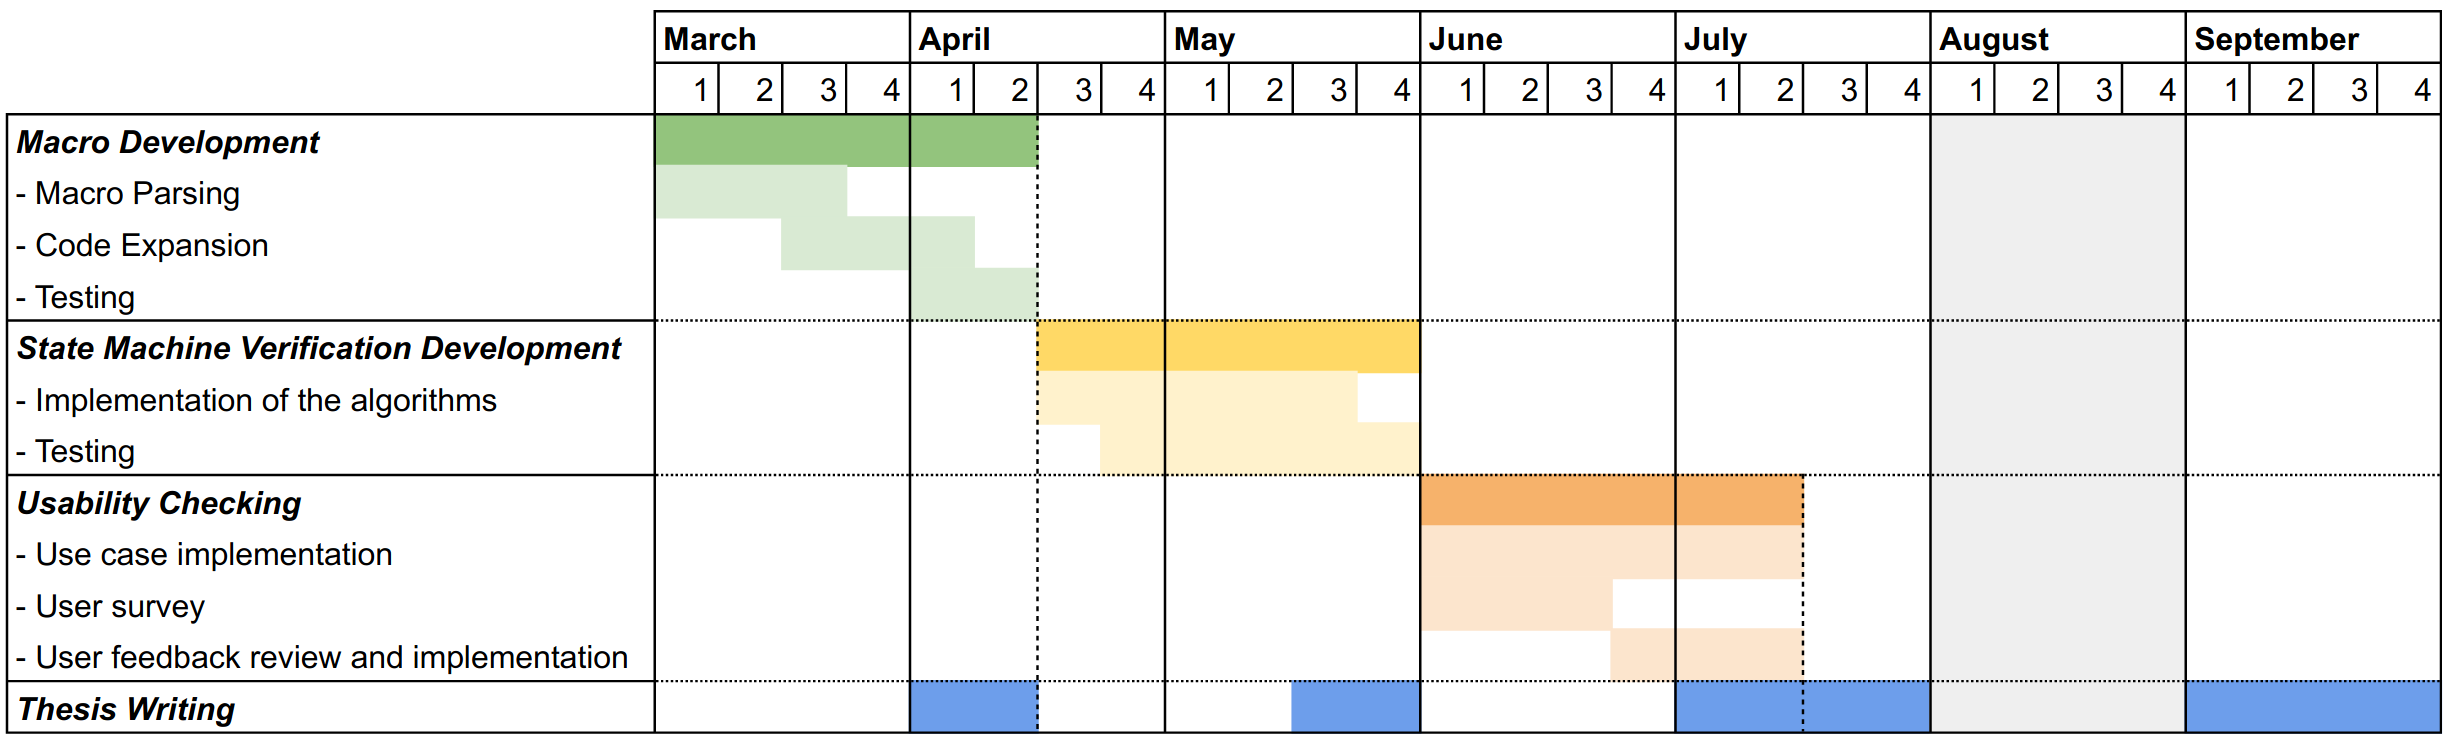
\includegraphics[width=\linewidth]{planning.png}
        \caption{Work plan Gantt chart}
    \end{figure}

    \note{
        \begin{pt}
            Por fim, apresento o plano de trabalho.

            (Apresentar e explicar a tabela.)
        \end{pt}
    }
\end{frame}

\end{document}